\chapter{Methodology}
In this chapter, the structure and implementation processes of the DDAE model (see section 3.1.1) and the Iterative Metric Learning model (see section 3.1.2) are presented in detail.

\section{Algorithm Implementation}
\subsection{DDAE}
In this section, the process of implementing the novel model DDAE\cite{73} is presented in detail from its four components. \textbf{Data Block Construction} is constructed to balance the class distribution. \textbf{Data Space Improvement} improves data space for the training set through \textbf{Largest Margin Nearest Neighbor(LMNN)}\cite{69}. \textbf{Adaptive Weight Adjustment} is inspired by cost-sensitive learning and it generates a weight to make the classifier work better. The last component, \textbf{Ensemble Learning}, utilizes major voting and the weight from Adaptive Weight Adjustment component to determine the ultimate prediction. In this algorithm, \textbf{\textit{k-nearest neighbors rule}}\textbf{(kNN)}\cite{75} will be used as the base classifier.

\subsubsection{Data Block Construction (DBC) Component}
The first step of DBC component is dividing the majority in the training set into several data blocks with a similar size compared to those in the minority in the training set. This can be viewed as an application of undersampling, due to the use of only some of majority samples. Each individually generated data block will be utilized as the training set for each base classifier of the ultimate ensemble classifier. As this approach is introduced to resolve class imbalance problem, the objective of this current component is to achieve better output for each base classifier through balancing the class distribution of each data block. Since one of the significant characteristics of an imbalanced dataset is the huge difference between the class sizes of the majority and minority, DBC applies the concept of oversampling to create more minority samples. This is achieved by copying all the minority samples and placing them in each data block.

Through this procedure, the issue of information loss and overfitting can be improved to some extent,mitigating the arguments against undersampling and oversampling.

The detail of the choice of the number of data blocks $\delta^{*}(\lceil\delta]$ or $\lfloor\delta\rfloor)$ is explained in Chapter 4.
\begin{algorithm}[h]
    \caption{Data Blocks Construction}
    \label{algo1}
    \hspace*{0.02in} {\bf Input:} Training Set $D_{t}$\\
    \hspace*{0.02in} {\bf Output:} A set $B$ of $\delta^{*}$ data blocks
    \begin{algorithmic}[1]
        \State Split the majority and minority instances in the training set into $S_{\text{maj}}$ and $S_{\min}$ respectively\newline Obtain the size of $S_{\text{maj}}$ and $S_{\min}$, denoted as $N_{\text{maj}}$ and $N_{\min}$\newline Obtain the balanced ratio $\delta=N_{\text{maj}} / N_{\min}$
        \State Initialize a set of blocks $B=\left\{B_{1}, B_{2}, \ldots, B_{\delta^{*}}\right\}$\newline $\left(\delta^{*}\right.$ can be considered as $\lceil\delta\rceil$ or $\lfloor\delta\rfloor)$
        \State Divide the majority samples into $\delta^{*}$ parts $\left\{M a_{1}, M a_{2}, \ldots, M a_{\delta^{*}}\right\}$
        \State Copy $S_{\min }$ and $M a_{i}$ into one of the empty data blocks $B_{i}$ which has been created in Step 2.
    \end{algorithmic}
\end{algorithm}

\subsubsection{Data Space Improvement (DSI) Component}
\begin{figure}[h]
    \centering 
    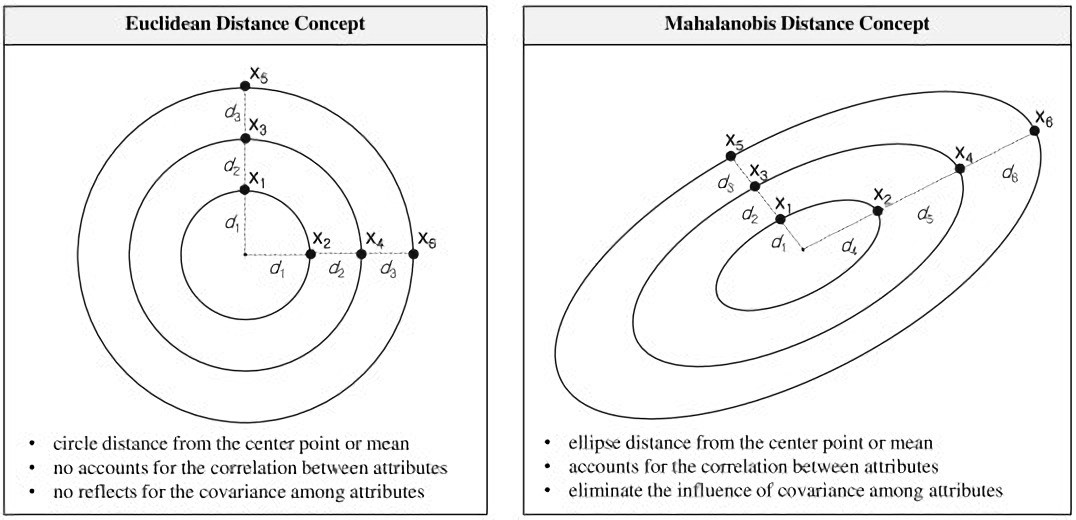
\includegraphics[width=\textwidth]{images/fig7}
    \caption{Comparison of Euclidean Distance and Mahalanobis Distance \cite[Fig.1]{76}}
    \label{fig7}
\end{figure}

In this component, a distance metrics learning algorithm called \textit{large margin nearest neighbor(LMNN)} \cite{69} is utilized to improve the data space for training samples in each data block generated in DBC component.

LMNN, first introduced by Kilian Q. Weinberger and Lawrence K. Saul in their 2009 work \cite{69}, absorbs the particular advantages of several individual models, such as Mahalanobis Metric for Clustering (MMC) [74], Pseudometric Online Learning Algorithm (POLA) \cite{65}, Neighborhood Component Analysis (NCA) \cite{71}. As the classification approach kNN is sensitive with the metric applied to calculate the distances between different examples, LMNN \cite{69} is proposed to learn \textbf{\textit{Mahalanobis distance metrics}} \cite{70} for kNN instead of Euclidean distances used by classical kNN. Figure \ref{fig7} illustrates the difference between these two kinds of distance metric algorithms. The Mahalanobis distance between two data instance points $x$ and $y$, is defined as
\begin{equation}\label{eq1}\footnotemark[1]
    D_{M}(x, y)=\sqrt{(x-y)^{T} \Sigma^{-1}(x-y)}
\end{equation}
\footnotetext[1]{Mahalanobis, P. C. (1936). On the generalized distance in statistics. National Institute of Science of India.}

This proposed approach contains three main parts: a convex loss function, an intention of maximizing margin and the constraints on the distance metric imposed by an accurate kNN algorithm. This, improves the classification accuracy of kNN significantly and it can even be comparable to the SVM classifier on some datasets.

Two simple objectives of LMNN defined in \cite{69} are:

for each training input sample $x_{i}$ and its label $y_{i}$,
\begin{enumerate}
    \item[1.] the label of its k nearest neighbors should be same with $y_i$
    \item[2.] the neighbors with different label should be separated widely. 
\end{enumerate}
\begin{figure}[h]
    \centering 
    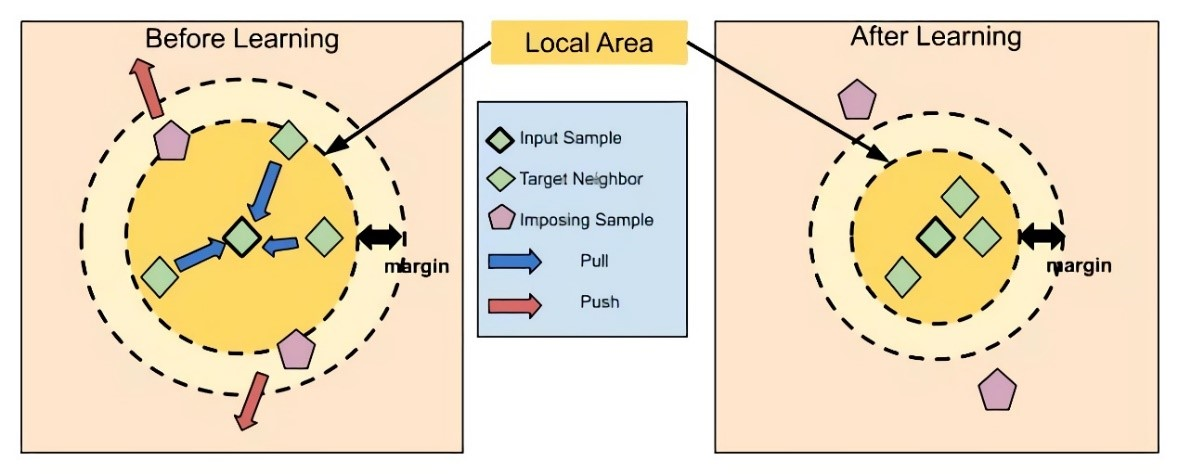
\includegraphics[width=\textwidth]{images/fig8}
    \caption{The procedure of LMNN Distance Metric Learning}
    \label{fig8}
\end{figure}

The first stage is, for each data sample $x_i$, to identify the \textit{target neighbors} that are desired to place close to $x_i$. In other words, there is specific ``margin'' around $x_i$, and other input samples with different labels should be placed further away, so the objective of learning is kind of minimization of the number of these imposing samples which can be introduced through an inequality:
\begin{equation}\label{eq2}\footnotemark[2]
    \left\|L\left(x_{i}-x_{p}\right)\right\|^{2} \leq\left\|L\left(x_{i}-x_{j}\right)\right\|^{2}+1
\end{equation}
\footnotetext[2]{Mahalanobis, P. C. (1936). On the generalized distance in statistics. National Institute of Science of India.}
, with $L$ a linear transformation \cite{69}. For instance, given an input sample $x_i$ with the class label $y_{i}$ and the target neighbor $x_{j}$, the imposing sample $x_{p}$ should satisfy the inequality. The detail of this procedure with $k=3$ as an example can be observed in Figure \ref{fig8}.

Accordingly, the overall loss function should contain two penalizing terms. One of them is used to limit large distances between neighboring input samples with the same class labels, by pulling target neighbors closer to $x_i$, the other is used to penalize small distances between neighboring input samples with different labels by pushing different labeled samples further away. In \cite{69}, the overall loss function for this distance metric learning is a combination of these two mentioned terms, which are denoted as $\varepsilon_{pull}(L)$ and $\varepsilon_{push}(L)$ respectively. With all the previous definitions, it is indicated that these two terms have competing effects, one for attracting the target neighbors and the other for avoiding or repelling the imposing samples. In order to balance these intentions, Weinberger and Saul gives a weighting parameter $\omega$, a positive real number, here. The overall loss function is defined as:
\begin{equation}\label{eq3}\footnotemark[3]
    \varepsilon(L)=(1-\omega) \varepsilon_{p u l l}(L)+\omega \varepsilon_{p u s h}(L)
\end{equation}
\footnotetext[3]{Weinberger, K. Q., \& Saul, L. K. (2009). Distance metric learning for large margin nearest neighbor classification. Journal of Machine Learning Research, 10(2).}
, with a general low-dependence on the value of $\mu$, which can be tuned with the help of cross-validation, for the result of minimizing the loss function.

The first term of loss function is defined as
\begin{equation}\label{eq4}\footnotemark[3]
    \varepsilon_{pull}(L)=\sum\limits_{j \sim i}\left\|L\left(x_{i}-x_{j}\right)\right\|^{2}
\end{equation}
, with $j \sim i$ denoted as each $x_{j},$ which is the target neighbor of $x_{i}$. It should be noted that this term only affects the input samples and their large-distancing target neighbors but not all other input samples with a same class label in the training set.

The second term of the loss function is given as (\ref{eq5})
\begin{equation}\label{eq5}\footnotemark[3]
    \varepsilon_{\text {push }}(L)=\sum\limits_{i, j \sim i} \sum\limits_{p}\left(1-\theta_{i p}\right) \max \left(1+\left\|L\left(x_{i}-x_{j}\right)\right\|^{2}-\left\| L\left(x_{i}-x_{p}\right)\right\|^{2}, 0\right)
\end{equation}
, where a new variable $y_{i p}$ is introduced to show whether the $x_{i}$ and $x_{p}$ belongs to the identified class. In particular, $\theta_{i p}=1$ if and only if $x_{i}$ and $x_{p}$ have the same class label, or $\theta_{i p}=0$. Additionally, the term $\max (m, 0)$ refers to the standard hinge loss. To be specific, if the input sample $x_{p}$ is placed away from $x_{i}$ safely, this means that its hinge loss is with a negative argument so that there will be no effect on the overall loss function. 

The last step of this approach is the minimization of this overall loss function. In \cite{69}, this can be achieved through gradient descent in the element of $L$.

\subsubsection{Adaptive Weight Adjustment (AWA) Component}
Since most ensemble learning approaches assume that the significance of each base classifier (or the weight of each base classifier) is totally equal \cite{32}, the purpose of this AWA component is to find an appropriate overall class weight generated using the data coming from each data block \cite{73}.

In \cite{73}, a definition called \textbf{\textit{unstable confusion matrix}} with a similar structure as classical confusion matrix (see Table \ref{tab2}) is first introduced in this component, which can be observed in Table \ref{tab4}. In detail, the figure for $u(0,0)($resp. $u(0,1))$ is the number of unstable samples with negative as real label and predicted as negative(resp. positive) and so the figure for $u(1,1)($resp. $u(1,0))$ represents the number of \textit{unstable samples} with positive as the real label and classified as positive(resp. negative).
\begin{table}[h]
    \centering
    \begin{tabular}{|c|c|c|}
    \hline
                     & Actual negative              & Actual positive              \\ \hline
    Predict negative & $u(0,0)$ (True Negative)     & $u(1,0)($ False Positive $)$ \\ \hline
    Predict positive & $u(0,1)($ False Positive $)$ & $u(1,1)$ (True Negative)     \\ \hline
    \end{tabular}
    \caption{Unstable Confusion Matrix}
    \label{tab4}
\end{table}

But how is an \textit{unstable sample} defined here? First, it should be noted that, as the kNN classifier is utilized as a base classifier in this DDAE model, it is probable that the k-nearest neighbors for each data sample are not labeled similarly \cite{73}. One particular instance of this is when the number of two class samples among these k neighbors is not very different. For instance, if $k$ is assumed as 7, and among the 7 nearest neighbors of a data sample $s$, there are 3 labeled as negative and the other 4 are labeled as positive. According to the kNN rule, these should be predicted as positive but in reality, this decision can be somewhat ambiguous. So this kind of data sample is called an unstable sample, and in \cite{73}, the absolute difference between the number of these two class samples, so-called \textbf{\textit{positive-negative count difference (PNCD)}}, is introduced to distinguish the unstable sample more formally:
\begin{equation}\label{eq6}\footnotemark[4]
    s \in\left\{\begin{array}{ll}
    \text {unstable samples, } & \text { PNCD }<\rho \\
    \text {stable samples, } & \text { otherwise }
    \end{array}\right., \text{ with }\rho=\left\{\begin{array}{ll}
        1, & k \text { is odd } \\
        2, & \text { otherwise }
        \end{array}\right..
\end{equation}
\footnotetext[4]{Yin, J., Gan, C., Zhao, K., Lin, X., Quan, Z., \& Wang, Z. J. (2020). A Novel Model for Imbalanced Data Classification. In AAAI (pp. 6680-6687).}

To determine PNCD for each test data sample, in each data block, the distances between the specific data sample and each sample in the data block are determined from Euclidean distances.

After finding $k$ nearest neighbors for each test sample, it is easy to calculate the PNCD for it. According to (\ref{eq6}), a judgement will be given as to whether this sample belongs to the set of unstable samples or not. 
\begin{algorithm}[h]
    \caption{Find Neighbors for Test Sample}
    \label{algo2}
    \hspace*{0.02in} {\bf Input:} Test Instance $t,$ Data Block $b_{j}$ with $q$ data samples\\
    \hspace*{0.02in} {\bf Output:} List $neigh$ with $k$ samples(neighbors) 
    \begin{algorithmic}[1]
        \State Initialize an empty lists $distance$
        \For{$j=0$ to $q-1$}
            \State Calculate the distance $dist_{j}$ between $b_{i}[j]$ and $t$
            \State Add ($dist_{j}, j$) into list $distance$
        \EndFor
        \State Sort the list $distance$ according to the first term of each tuple in $distance$
        \For{$z=0$ to $k-1$}
            \State Add $b_{i}\left[\text{distance}\left[z\right]\left[1\right]\right]$ into $neigh$
        \EndFor
        \State \textbf{return} $neigh=\left\{neigh_{0}, neigh_{1}, \ldots, neigh_{k-1}\right\}$
    \end{algorithmic}
\end{algorithm}

As discussed in Chapter 2, the cost of the class positive (minority) is generally higher or more expensive than that of class negative (majority) in imbalanced binary classification. AWA works on the adjustment of weights for the positive and negative predictions and the maximization of the overall gain $g_{overall}$ for the unstable confusion matrix \cite{73}. The weight pair $Weight=\left(Weight_{n}, Weight_{p}\right)$ consists of the weights for negative predictions and positive predictions. $Weight$ is set to $\left(Weight_{\text {default}}, Weight_{\text {default}}\right)$ initially with $Weight_{\text{default}}=1$. If there is an increase with the weights for class positive(resp. negative), $g_{p}\left(\text{resp. } g_{n}\right), g_{\text {overal }}$ is set to $g_{p}\left(\text{resp. } g_{n}\right)$. Otherwise $g_{overall}$ is set to $g_d$.
\begin{equation}\label{eq7}\footnotemark[4]
    \left\{ 
        \begin{array}{l}
            g_{d}=x *(u(1,1)-u(1,0))+(u(0,0)-u(0,1))\\ 
            g_{p}=x *(u(1,1)+u(1,0)+(-u(0,0)-u(0,1))\\ 
            g_{n}=x *(-u(1,1)-u(1,0)+u(0,0)+u(0,1))
        \end{array}    
    \right.
\end{equation}
\footnotetext[4]{Yin, J., Gan, C., Zhao, K., Lin, X., Quan, Z., \& Wang, Z. J. (2020). A Novel Model for Imbalanced Data Classification. In AAAI (pp. 6680-6687).}

In order to maximize the $g_{overall}$, the next step is to find the maximal figure among these three gains. The weight pair $Weight=\left(Weight_{default}, Weight_{default}\right)$ will be updated through a new weight $Weight_{new}=Weight_{threshold}+\gamma$ as follow:
\begin{table}[h]
    \centering
    \begin{tabular}{|c|l|}
    \hline
    $g_d$ maximal: & $Weight=\left(Weight_{default}, Weight_{default}\right)$ \\ \hline
    $g_p$ maximal: & $Weight=\left(Weight_{default}, Weight_{new}\right)$     \\ \hline
    $g_n$ maximal: & $Weight=\left(Weight_{new}, Weight_{default}\right)$     \\ \hline
    \end{tabular}
    \caption{Updating Weight Pair}
    \label{tab5}
\end{table}

with $\gamma$ a small real number larger than 0 and $Weight_{threshold}$ defined as (\ref{eq8})
\begin{equation}\label{eq8}\footnotemark[4]
    Weight_{threshold}=\left\{\begin{array}{ll}
        \hspace{-6pt}\dfrac{\lfloor \frac{\delta^{*}}{2}\rfloor +1}{\lfloor \frac{\delta^{*}}{2}\rfloor -1}, & \text { if } \delta^{*} \text { is odd } \\
    \hspace{-6pt}\dfrac{\frac{\delta^{*}}{2}+1}{\frac{\delta^{*}}{2}-1}, & \text { otherwise }
    \end{array}\right.
\end{equation}
\footnotetext[4]{Yin, J., Gan, C., Zhao, K., Lin, X., Quan, Z., \& Wang, Z. J. (2020). A Novel Model for Imbalanced Data Classification. In AAAI (pp. 6680-6687).}
\begin{algorithm}[h]
    \caption{Determination of overall weight pair}
    \label{algo3}
    \hspace*{0.02in} {\bf Input:} threshold\ $\tau$, $\#default\ weight\ pairs$\footnotemark[5]

    $\hspace{35pt} \#positive\ weight\ pairs$\footnotemark[6], $\#negative\ weight\ pairs$\footnotemark[7]

    $\hspace{35pt}\#all\ weight\ pairs$\footnotemark[8] \\
    \hspace*{0.02in} {\bf Output:} Overall weight pair $Weight^{overall}$
    \begin{algorithmic}[1]
        \If{$\#default\ weight\ pairs\ / \#all\ weight\ pairs\geq \tau$}
            \State \textbf{return} ($Weight_{default},Weight_{default}$)
            \Else
            \If{$\#positive\ weight\ pairs >\#negative\ weight\ pairs$}
                \State \textbf{return} ($Weight_{new},Weight_{default}$)
                \Else
                \State \textbf{return} ($Weight_{default},Weight_{new}$)
            \EndIf
        \EndIf
    \end{algorithmic}
\end{algorithm}
\footnotetext[5]{The number of default weight pairs($Weight_{default},Weight_{default}$)}
\footnotetext[6]{The number of non-default positive weight pairs($Weight_{new},Weight_{default}$)}
\footnotetext[7]{The number of non-default negative weight pairs($Weight_{new},Weight_{default}$)}
\footnotetext[8]{The number of all weight pairs $= 5 + 6 + 7$}

After finishing the above steps, for a single test sample, the result will be $\#data\ block$\footnotemark[9] weight pairs obtained from each data block. The last step(see Algorithm \ref{algo3}) of AWA component is to determine the final overall weight pair $Weight^{overall}=\left(Weight_{n}^{overall},Weight_{p}^{overall}\right)$ for this single test sample, which depends on the frequency of these three different kinds of weight pairs shown in Table \ref{tab5}.
\footnotetext[9]{The number of data blocks}

\subsubsection{Ensemble Learning Component (EL) Component}
The main idea behind this component is ensemble learning (see section 2.2.3), with a weighting parameter determined in AWA component. Multiple base classifiers with major voting technique work on the final decision for each input sample. The number of base classifiers $m$ in this ensemble classifier depends on the number of data blocks generated in DBC component, so is $m=\delta^{*}$.

In particular, this paper focuses on binary classification. At the first stage, for each sample $s$ that needs to be predicted, the number of base classifiers that have predicted it as positive (class label 1) and those as negative (class label 0) need to be counted respectively. This can be denoted as a term $\left(n_{1}, n_{0}\right)$. Namely, for the \textit{i}th base classifier $C L_{i}$, the $r_{(i, label)}(s)=1$ if, and only if, the predicted label for $s$ that made by $C L_{i}$ is same as $label$, with $i$ in range of 0 to $m-1$ and $label\in\{0,1\}$. With this, it is easy to obtain $n_{1}=\sum_{i=0}^{m-1} r_{(i, 1)}(s)$ and $n_{0}=\sum_{i=0}^{m-1} r_{(i, 0)}(s)$.

As introduced in section 2.1.1, the minority or positive class in a class imbalanced dataset always has more impact than the majority or negative class. In order to solve this problem and to enhance the performance of the ensemble classifier, the overall weight $Weight^{overall}=\left(Weight_0^{overall},Weight_1^{overall}\right)$ is utilized to balance these two classes. Thus, the modified major voting technique can be defined as (\ref{eq9}).
\begin{equation}\label{eq9}\footnotemark[10]
    Res(s)=\left\{\begin{array}{ll}
    \hspace{-6pt}label_{0}, & Weight_{0}^{overall} * n_{0} \geq Weight_{1}^{overall} * n_{1} \\
    \hspace{-6pt}label_{1}, & otherwise
    \end{array}\right.
\end{equation}
\footnotetext[10]{Yin, J., Gan, C., Zhao, K., Lin, X., Quan, Z., \& Wang, Z. J. (2020). A Novel Model for Imbalanced Data Classification. In AAAI (pp. 6680-6687).}

\subsection{Iterative Metric Learning(IML)}
In this section, the process of implementing the model IML \cite{72} is presented in detail with its three components. \textbf{Iterative Metric Learning} is constructed to improve the structure of data space through \textbf{Largest Margin Nearest Neighbor(LMNN)} \cite{69}. \textbf{Iterative Training Samples Selection} finds the samples which are more likely to affect the testing data samples. \textbf{Data Matching} determines the most effective neighborhood for each testing data sample. In this algorithm, \textbf{k-nearest neighbors rule(kNN)} \cite{75} will be used as the base classifier. Algorithm \ref{algo4} shows the detail in dealing with imbalanced datasets through IML.

\subsubsection{Iterative Metric Learning}
In this stage, IML also utilizes the LMNN, which was explained in last section, to improve the data space. The objective of this component is same as that of DSI in DDAE, both of which want to separate the data samples with a different class label by a large margin and make the samples with the same class labels close to each other. Unlike DDAE, IML provides an iterative metric learning approach which can locate a more stable neighborhood for the specific testing data.

\subsubsection{Iterative Training Samples Selection}
In this stage, after calculating the distance between each of the samples from training set and the to-be-classified testing sample, the top $d^{p}$ and the top $d^{f}$ training samples for the positive and negative class will be selected; these chosen samples make up the sub training set for the current testing sample \cite{72}.

\subsubsection{Data Matching}
After the first two steps, a temporary neighborhood for the current testing sample has already been discovered. However, to find the most effective training set for the testing sample, the first two steps need to be iteratively repeated. In each iteration, the current discovered neighborhood will be compared with the previously discovered neighborhood. If the ratio between the number of matched training samples and the number of all training samples is greater than the matching ratio, this means that the neighborhood is already stable and the current neighborhood is the appropriate training set for this current testing sample, or the iteration needs to continue until the above condition is met.
\begin{algorithm}[h]
    \caption{IML}
    \label{algo4}
    \hspace*{0.02in} {\bf Input:} Testing set $S^{test}$, Training Set $S^{train}$, matched ratio $\beta$, kNN Classifier $K$\\
    \hspace*{0.02in} {\bf Output:} List of predictions for the given testing set $P$
    \begin{algorithmic}[1]
        \For{$s^{test}$ in $S^{test}$}
            \State Initialize $Pre\_set$ and $Curr\_Set$
            \While{true}
                \State do Metric Learning on $S^{train}$ and update $S^{train}$
                \State do Training Samples Selection and update the $Curr\_Set$
                \State do Data Matching and find the matched samples
                \If{\#matched samples / size$(Curr\_Set) >=\beta$}
                    \State trained the $K$ using $Curr\_Set$, add the prediction into $P$
                    \State \textbf{break}
                    \Else\State $Pre\_set = Curr\_Set$
                \EndIf
            \EndWhile
        \EndFor
        \State \textbf{end for}
        \State \textbf{return} $P$
    \end{algorithmic}
\end{algorithm}